% AAAI-style layout (two columns, Times, 7in x 9.25in text block) rebuilt with article: the official aaai*.sty is not installed here.
\documentclass[letterpaper,10pt,twocolumn]{article}
\usepackage[letterpaper,textwidth=7in,textheight=9.25in,columnsep=0.33in,top=0.75in]{geometry}
\usepackage{times,helvet,courier}
\usepackage[T1]{fontenc}
\usepackage{amsmath,booktabs,graphicx,tabularx,xcolor,caption}
\usepackage{natbib}
\usepackage[hidelinks]{hyperref}
\captionsetup{font=small,labelfont=bf}
\setlength{\parskip}{0pt}
\renewcommand{\arraystretch}{1.08}
\makeatletter
\renewcommand\section{\@startsection{section}{1}{\z@}{-1.6ex plus -.4ex}{0.8ex}{\normalfont\large\bfseries\centering}}
\renewcommand\subsection{\@startsection{subsection}{2}{\z@}{-1.2ex plus -.3ex}{0.5ex}{\normalfont\normalsize\bfseries}}
\renewcommand\paragraph{\@startsection{paragraph}{4}{\z@}{0.6ex plus .2ex}{-1em}{\normalfont\normalsize\bfseries}}
\makeatother

\title{\Large\bfseries Deep Learning Project 1}
\author{Chetan Kodeboyina (ck3399) \quad Shwetanshu Raj (sr8250) \quad Ninad Rade (nr3263)\\ Team \textit{Jugaad Net} \\ New York University, ECE-GY 7123 Deep Learning, Project 1}
\date{}

\begin{document}
\maketitle

\begin{abstract}
We train a residual network with fewer than 5M parameters from scratch on the 50,000 CIFAR-10 training images and predict a hidden 2,000-image test set drawn from a newer, shifted collection of images. Our final model is a 4.70M-parameter ResNet trained for 400 epochs with CutMix, blur and zoom-out augmentation, and distillation from four same-size teachers. Over about 30 training runs and 33 submissions the public score rose from 0.874 to 0.911. This report describes the ideas we tested and what we learned. Most of the gain came from using all the data, the full parameter budget and enough epochs. Held-out accuracy on training images was close to 98.5\% for every variant and did not predict the leaderboard. Each half of the test set, about 1,000 images, was too small to rank models this close. Our selected 0.911 submission scored 0.876 on the private half (rank 22), below seven submissions we did not choose, yet it is the most accurate of all our submissions on the full 2,000 images. Averaged over seeds on the full test set, the basics account for 0.021 of the 0.025 total gain. Distillation and the shift-targeted augmentation together add 0.004, which is within noise.
\end{abstract}

\section{Introduction}
The task is CIFAR-10 classification \citep{krizhevsky2009} under three rules: a single model, at most 5M trainable parameters, trained from scratch with no external data. Models are scored on 2,000 hidden images, 200 per class. The public leaderboard uses about half of them, so each image is worth 0.001 of accuracy.

What makes the task hard is that the hidden images come from a newer collection than the training images. \citet{recht2018} showed that such a collection, gathered the same way, costs CIFAR-10 models several points of accuracy for reasons that are not fully understood. Our models score about 98.5\% on held-out training images but only about 0.89 on the hidden test set. So most of our work was about making a small model hold up on slightly different photos.

All local measurements in this report use a fixed 5,000-image held-out split of the training set, on models trained with the other 45,000 images. The hidden test images were never used for training or for choosing between models.

\paragraph{Main takeaways.}
\begin{itemize}\setlength{\itemsep}{1pt}
\item Most of the gain came from the basics. All 50k images, a network deep enough to use the parameter budget, CutMix and 400 epochs took the public score from 0.874 to 0.899.
\item Blur and zoom-out augmentation, aimed at the shift, produced our best public score, 0.911. Averaged over seeds on the full test set the gain is about 0.004, which is within noise.
\item Longer training, larger teachers and stronger augmentation all scored lower.
\item Held-out accuracy did not track the leaderboard, and seed variance ($\pm$0.01) was as large as the effects we were measuring.
\item Public score did not predict private score. Seven submissions we did not select beat our pick on the private half, but our pick was the most accurate on the full test set.
\end{itemize}

\section{The Recipe in Brief}
We kept the model family fixed and spent our effort on data, training and evaluation. The network is a standard basic-block ResNet \citep{he2016}: a 64-channel stem and three stages of 64, 128 and 256 channels with 4, 4 and 3 blocks, global average pooling and a linear layer (4,697,162 parameters, Table~\ref{tab:arch}). Training uses SGD with cosine learning-rate decay \citep{loshchilov2017}, weight averaging (EMA), label smoothing \citep{szegedy2016} and four kinds of augmentation:
\begin{itemize}\setlength{\itemsep}{1pt}
\item \textbf{General:} random crops and flips, TrivialAugment \citep{muller2021} and small random erasing \citep{zhong2020}.
\item \textbf{Mixing:} CutMix \citep{yun2019}, which pastes a patch of one image into another and mixes the labels.
\item \textbf{Shift-targeted:} Gaussian blur on 20\% of images and zoom-out on 30\%, which shrinks the object inside the frame.
\item \textbf{Distillation:} the model learns to match the averaged predictions of four same-size teachers, following the ``patient and consistent'' setup of \citet{beyer2022}.
\end{itemize}
At test time we average predictions over the image, its mirror image and small shifts.

\begin{table}[t]
\centering\small
\begin{tabular}{lccc}
\toprule
Stage & Channels & Blocks & Feature map \\
\midrule
Stem & 64 & -- & $32\times32$ \\
Stage 1 & 64 & 4 & $32\times32$ \\
Stage 2 & 128 & 4 & $16\times16$ \\
Stage 3 & 256 & 3 & $8\times8$ \\
Pool + linear & 10 & -- & $1\times1$ \\
\midrule
\multicolumn{4}{l}{Parameters: \textbf{4,697,162} of 5,000,000 allowed}\\
\bottomrule
\end{tabular}
\caption{Final architecture: basic residual blocks with $3\times3$ kernels.}
\label{tab:arch}
\end{table}

\section{Attempts Made}
Figure~\ref{fig:progress} shows the five steps that raised the public score. The scores in this section are public scores. Section~\ref{sec:noise} revisits each step with seed averages on the full test set.

\begin{figure}[t]
\centering
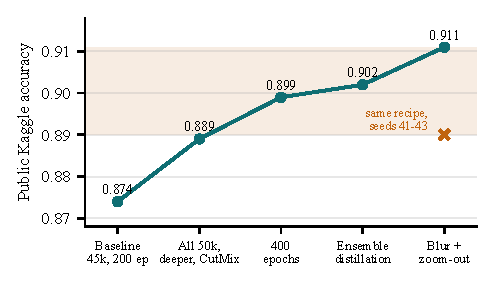
\includegraphics[width=\columnwidth]{figs/progress.pdf}
\caption{Best public score after each milestone. Crosses: the final recipe rerun with seeds 42 and 43. The shaded band is the spread of that one recipe across three seeds.}
\label{fig:progress}
\end{figure}

\paragraph{Use everything we are allowed (0.874 $\to$ 0.889).} Our baseline held out 5k images for validation and used a (3,3,3) network. Training on all 50k images, adding blocks up to the 5M budget and adding CutMix gave the largest single jump. Before trying more complex ideas, it is worth using all the data and all the capacity the rules allow.

\paragraph{Train longer (0.889 $\to$ 0.899).} Doubling training from 200 to 400 epochs added a full point. Going further did not: 600, 800 and 1,200 epochs all scored at or below 400. Figure~\ref{fig:curve} shows where the gain comes from. Held-out accuracy rises from 95.7\% at epoch 200 to 98.5\% at epoch 400, almost all of it while the cosine schedule lowers the learning rate, and the training loss falls in step. A longer schedule only spreads this late improvement over more epochs.

\begin{figure}[t]
\centering
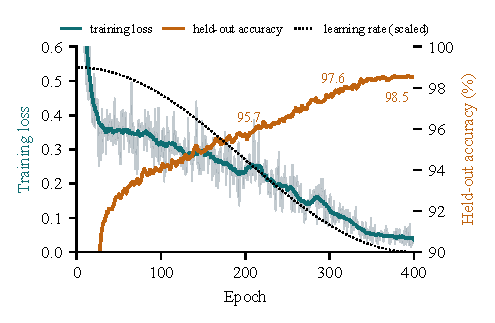
\includegraphics[width=\columnwidth]{figs/curve.pdf}
\caption{Training loss (smoothed; raw values in grey) and held-out accuracy of the final recipe trained on 45k images, evaluated each epoch on the 5k images it never trained on (EMA weights, image + mirror). Most of the held-out gain comes in the second half, as the learning rate decays.}
\label{fig:curve}
\end{figure}

\paragraph{Learn from an ensemble (0.899 $\to$ 0.902).} An ensemble of models is more accurate than any one of them, but the rules allow only a single model. Distillation lets one model learn the ensemble's averaged predictions. The version that worked used soft targets only (no hard labels) and showed the teachers the same augmented image as the student \citep{beyer2022}. Earlier variants scored lower, including a higher temperature (0.888) and teachers that never saw the image they labelled (0.875). Once the private scores were known, this step turned out to be within noise (Section~\ref{sec:noise}).

\paragraph{Target the shift (0.902 $\to$ 0.911).} We measured how our models fail on degraded images (Section~\ref{sec:shift}) and found two weak spots: blur and small objects. Adding blur and zoom-out to training produced our best public score.

\paragraph{Check the result (0.911 $\to$ 0.895).} At the end we reran the exact 0.911 recipe with two new seeds. They scored 0.895 and 0.898. This changed how we interpret the other results (Section~\ref{sec:noise}).

\section{Probing Robustness and Errors}
\label{sec:shift}
Because newer photos can differ in sharpness and framing, we asked how the model copes with degraded versions of images it has never seen. All numbers in this section use the 5,000 held-out training images and models trained on the other 45,000.

\paragraph{Distortion tests.} We applied controlled distortions (Figure~\ref{fig:distort}) and measured accuracy. Without the shift-targeted augmentation, the distilled model dropped from 98.4\% to 83.7\% under blur ($\sigma$=1.2) and to 79.1\% when the object filled only 16 pixels. Dogs and cats suffered most under blur (63.5\% and 72.7\%). Adding blur and zoom-out to training raised these to 86.9\% and 81.9\% while leaving clean accuracy unchanged (Figure~\ref{fig:robust}). On the public leaderboard the same change was worth 0.009, from 0.902 to 0.911. Averaged over seeds on the full test set it is worth about 0.004 (Section~\ref{sec:noise}).

\begin{figure}[t]
\centering
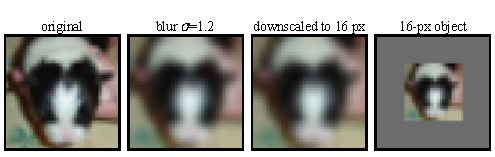
\includegraphics[width=\columnwidth]{figs/distortions.pdf}
\caption{The distortion tests applied to a held-out training image.}
\label{fig:distort}
\end{figure}

\begin{figure}[t]
\centering
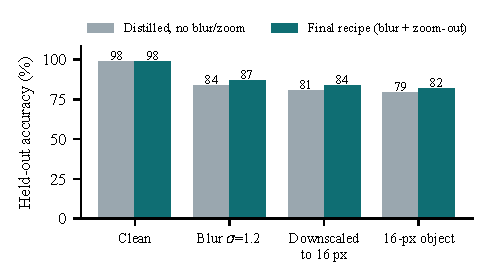
\includegraphics[width=\columnwidth]{figs/robust.pdf}
\caption{Held-out accuracy (single view) of the distilled model before and after adding blur and zoom-out augmentation. Robustness improves without any cost on clean images.}
\label{fig:robust}
\end{figure}

\paragraph{Error analysis.} The final recipe makes 68 errors on the 5,000 held-out images (98.6\% with test-time averaging). Figure~\ref{fig:conf} counts the most common confusions and Figure~\ref{fig:examples} shows the most confident ones. Cat and dog account for 25 of the 68. The rest are spread thinly across many pairs, mostly small or partly hidden animals and unusual viewpoints. Many of the confident mistakes are hard even for a person at 32$\times$32 pixels.

\begin{figure}[t]
\centering
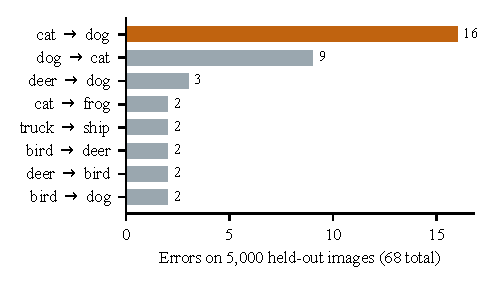
\includegraphics[width=\columnwidth]{figs/confusions.pdf}
\caption{Most frequent confusions of the final recipe on the held-out images. Cat and dog are the largest group.}
\label{fig:conf}
\end{figure}

\begin{figure}[t]
\centering
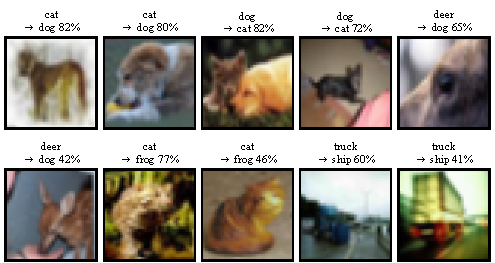
\includegraphics[width=\columnwidth]{figs/examples.pdf}
\caption{The most confident held-out errors for the main confusion pairs (true class $\to$ prediction, confidence).}
\label{fig:examples}
\end{figure}

\paragraph{The limit of held-out data.} Held-out images come from the same collection as the training images, so they cannot show what is different about the hidden set. Every distilled variant we trained on 45k images landed between 98.5\% and 98.7\% held-out, while the same variants differed by up to 0.02 on the leaderboard.

\section{Ideas Pursued}
Besides the milestones above, we followed six lines of work. Each started from a specific hypothesis.
\begin{enumerate}\setlength{\itemsep}{1pt}
\item \textbf{More capacity per parameter.} A wider, shallower network and a Shake-Shake network \citep{gastaldi2017} might use the 5M budget better than a standard ResNet.
\item \textbf{Better optimization.} Sharpness-aware minimization \citep{foret2021} seeks flatter minima, which some work suggests transfer better to new data.
\item \textbf{Better teachers.} If distillation helps, a stronger teacher should help more: we tried a 36.7M-parameter teacher, nine teachers, and teachers that were themselves distilled.
\item \textbf{Other augmentations.} AugMix \citep{hendrycks2020}, Cutout \citep{devries2017}, grayscale and stronger blur and zoom each target a different kind of robustness.
\item \textbf{Different mixing.} ResizeMix \citep{qin2020} pastes a whole shrunken image instead of a patch, so the pasted object is always complete; zoom-in crops target close-up views.
\item \textbf{Teacher-free robustness.} Teachers trained without blur might hold the student back, so we trained blur-augmented models without teachers and distilled from those.
\end{enumerate}
None of these improved the public score. The next three sections explain why we think so.

\section{Results}
Table~\ref{tab:local} summarizes the main models and Figure~\ref{fig:uploads} shows every submission. Held-out accuracy, where we have it, barely moves. The public leaderboard spans 0.874 to 0.911 and the private one 0.851 to 0.882. Table~\ref{tab:full} in Section~\ref{sec:noise} gives seed averages on the full test set, which is the most reliable comparison we have.

\begin{table}[t]
\centering\small
\setlength{\tabcolsep}{2.6pt}
\begin{tabular}{lcccc}
\toprule
Model & Held-out & Public & Private & All \\
\midrule
Baseline (3,3,3), 200 ep & 97.22 & 0.874 & 0.851 & 0.863 \\
Distilled, 4 teachers & 98.56 & 0.902 & 0.871 & 0.887 \\
\textbf{Final (blur + zoom-out)} & \textbf{98.64} & \textbf{0.911} & 0.876 & \textbf{0.894} \\
\quad same, seed 42 & -- & 0.895 & 0.877 & 0.886 \\
\quad same, seed 43 & -- & 0.898 & 0.869 & 0.884 \\
\quad 800 epochs & -- & 0.902 & 0.876 & 0.889 \\
\quad no CutMix & -- & 0.895 & 0.866 & 0.881 \\
\quad ResizeMix & -- & 0.897 & 0.877 & 0.887 \\
Shake-Shake, 1800 ep & -- & 0.897 & \textbf{0.878} & 0.888 \\
\bottomrule
\end{tabular}
\caption{Held-out accuracy (\%, 5k images, models trained on 45k, test-time averaging), with the public and private scores of the matching model trained on all 50k. ``All'' is the mean of public and private, the accuracy on all 2,000 test images. ``--'': no 45k version was trained.}
\label{tab:local}
\end{table}

\begin{figure*}[t]
\centering
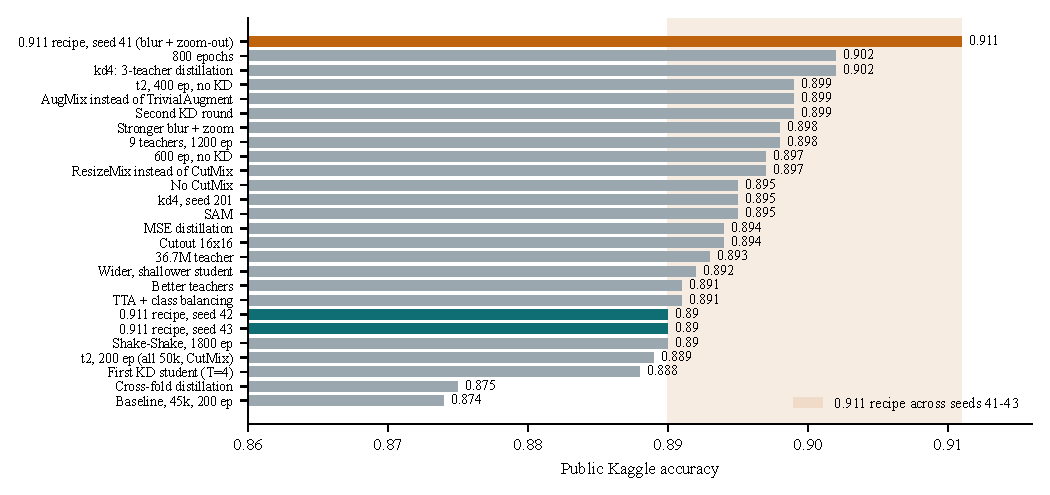
\includegraphics[width=\textwidth]{figs/uploads.pdf}
\caption{Public score of every scored submission. The shaded band is the spread of the final recipe across seeds 41--43 (0.895 to 0.911); most variants fall inside it. Not shown: grayscale augmentation (no gain, score not recorded) and seven early submissions without a recorded description.}
\label{fig:uploads}
\end{figure*}

\section{What We Expected to Work but Didn't}
Table~\ref{tab:fail} lists the ideas we were most confident about. We see three patterns.

\begin{table}[t]
\centering\small
\setlength{\tabcolsep}{3pt}
\begin{tabularx}{\columnwidth}{@{}>{\raggedright\arraybackslash}Xc>{\raggedright\arraybackslash}p{3.0cm}@{}}
\toprule
Idea & Public & Outcome \\
\midrule
600 / 800 / 1200 epochs & .897/.902/.898 & Never better than 400 \\
36.7M or better teachers & .893/.891 & Stronger teacher, weaker student \\
Sharpness-aware min. & .895 & No gain, twice the cost \\
Stronger blur + zoom & .898 & Too much distortion \\
Shake-Shake, 1800 ep & .897 & Strong on paper, no gain \\
ResizeMix & .897 & No gain over CutMix \\
Grayscale & no gain & +0.06 held-out only \\
Other distillation variants & .875--.899 & None beat the simple version \\
Balancing class counts & .891 & Below plain averaging (0.899) \\
\bottomrule
\end{tabularx}
\caption{Ideas we expected to help, with public scores.}
\label{tab:fail}
\end{table}

\paragraph{Pushing working ideas further did not help.} Longer training, more teachers and stronger augmentation had each helped in a mild form. Pushed further, they did as well on the training distribution but gave no measurable gain on the hidden set.

\paragraph{Stronger teachers gave weaker students.} A 36.7M-parameter teacher reached 97.84\% held-out after only 200 epochs, but its student scored 0.893, below students of our same-size teachers. One possible reason is that a small student finds it harder to match a much larger, very different network.

\paragraph{Targeted fixes were too small to see.} ResizeMix, zoom-in and teacher-free distillation each aimed at a narrow kind of error. Even if they worked, they would change only a handful of the 1,000 public images, below the noise floor of one submission.

\section{How Much Was Noise}
\label{sec:noise}
\paragraph{Seeds.} Rerunning the final recipe with seeds 42 and 43 scored 0.895 and 0.898, against 0.911 for seed 41 (Figure~\ref{fig:seeds}). An earlier recipe varied by 0.005 across three seeds. Two seeds of the same recipe disagree on 72--80 of the 2,000 hidden images. That is more than our 800-epoch run (58) or ResizeMix run (68) changed relative to 0.911. So most of the variants in Table~\ref{tab:fail} were compared against a high draw, and some may be as good as the recipe's typical result.

\begin{figure}[t]
\centering
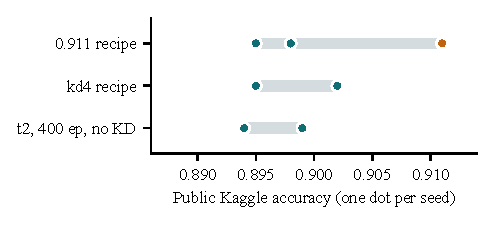
\includegraphics[width=\columnwidth]{figs/seeds.pdf}
\caption{Public score of the same recipe with different seeds. The final recipe spans 0.016, the size of most effects we tried to measure.}
\label{fig:seeds}
\end{figure}

\paragraph{Public versus private.} After the competition, Kaggle revealed each submission's score on the other half of the hidden set. We had chosen our two final submissions by public score: 0.911 and 0.902, the two highest. On the private half both scored 0.876, which ranked us 22nd (16th on public). Seven submissions we did not choose scored higher, the best at 0.882 (Figure~\ref{fig:private}). Excluding our two earliest and weakest runs, the rank correlation between public and private score across the other 31 submissions is only 0.18 ($p=0.34$). The private half is harder for every submission, about 0.024 lower on average, but the order of our models within it is close to random.

\paragraph{Why unselected submissions scored higher.} We do not think those seven were better models. Each half has about 1,000 images, so a single score has a standard error of about 0.010, and the best private score is only six images above our pick. The highest score on either half is partly the luckiest one (the winner's curse). Our 0.911 was lucky on the public half, and the submissions that beat it on private were lucky on the private half. They had ordinary public scores of 0.891 to 0.898. Averaging the two halves gives accuracy on all 2,000 images, with a standard error near 0.007. By that measure our selected submission is the best of all 33 at 0.8935, ahead of the best private scorer at 0.890 (Figure~\ref{fig:private}). Choosing by public score therefore did pick our most accurate submission. Its public score is 0.018 above its full-set accuracy, against 0.012 for a typical submission, so roughly 0.006 of the 0.911 was luck on the public half.

\paragraph{What the full test set says about each step.} With both halves known, we can average seeds over 2,000 images (Table~\ref{tab:full}). One model's accuracy on 2,000 images has a standard error of about 0.007, and the three seeds of the final recipe range from 0.884 to 0.894, so differences of a few thousandths are within noise. The basics account for 0.021 of the 0.025 total gain, and this is the only part that is clearly larger than the noise. Distillation adds 0.001 and blur with zoom-out 0.004. Both are too small to distinguish from zero with two or three seeds, and both are smaller than the public leaderboard suggested (0.003 and 0.009). Removing CutMix costs 0.007, and 800 epochs, ResizeMix and Shake-Shake all land within about 0.001 of the final recipe's average.

\begin{table}[t]
\centering\small
\setlength{\tabcolsep}{3.5pt}
\begin{tabular}{lcccc}
\toprule
Recipe & Seeds & Public & Private & All 2,000 \\
\midrule
Baseline, 45k, 200 ep & 1 & 0.874 & 0.851 & 0.863 \\
+ all data, depth, CutMix & 1 & 0.889 & 0.866 & 0.878 \\
+ 400 epochs & 3 & 0.897 & 0.869 & 0.883 \\
+ distillation & 2 & 0.899 & 0.870 & 0.884 \\
+ blur and zoom-out & 3 & 0.901 & 0.874 & \textbf{0.888} \\
\midrule
Final recipe, no CutMix & 1 & 0.895 & 0.866 & 0.881 \\
Final recipe, 800 epochs & 1 & 0.902 & 0.876 & 0.889 \\
Final recipe, ResizeMix & 1 & 0.897 & 0.877 & 0.887 \\
Shake-Shake, 1800 ep & 1 & 0.897 & 0.878 & 0.888 \\
\bottomrule
\end{tabular}
\caption{Scores averaged over seeds. ``All 2,000'' is the mean of the public and private scores, which is the accuracy on the whole hidden test set. Differences below about 0.007 are within noise.}
\label{tab:full}
\end{table}

\begin{figure}[t]
\centering
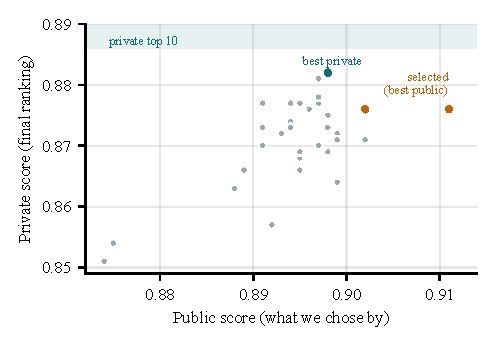
\includegraphics[width=\columnwidth]{figs/private.pdf}
\caption{Public against private score for all 33 submissions. The two we selected had the best public scores but only average private scores. Points on the dashed line have the same accuracy on all 2,000 images as our selected submission; no submission lies above it. Shaded: the private score needed for the top 10.}
\label{fig:private}
\end{figure}

\paragraph{Held-out accuracy.} Our held-out split is saturated. The distilled variants we trained on 45k images differ by at most 0.15 points, about the noise of 5,000 images, while their full-data versions differ by up to 0.02 on the leaderboard. For example, grayscale augmentation was 0.06 points better held-out but gave no gain on the leaderboard.

\section{What Surprised Us}
\begin{itemize}\setlength{\itemsep}{1pt}
\item \textbf{Our best public score was partly luck.} The same recipe scored 0.911, 0.895 and 0.898 on public, and 0.876, 0.877 and 0.869 on private.
\item \textbf{The private ranking was as noisy as the public one.} Seven unselected submissions beat our pick on the private half, but our pick was the most accurate on the full test set.
\item \textbf{Distillation, our most complex component, added almost nothing.} Averaged over seeds on the full test set it is worth 0.001.
\item \textbf{Robustness gains held-out did not carry over to the test set.} Blur and zoom-out added 3 points under blur on held-out images but only about 0.004 on the full test set, which is within noise.
\item \textbf{Bigger was not better.} A teacher seven times larger gave a weaker student, and training two or three times longer gave no gain.
\item \textbf{Cat and dog stayed the hardest pair.} They account for over a third of the final recipe's held-out errors, more than any augmentation changed.
\end{itemize}

\section{Lessons Learned}
\begin{enumerate}\setlength{\itemsep}{1pt}
\item \textbf{Measure the noise first.} One rerun with a new seed, done early, would have shown that differences under 0.02 cannot be read from a single submission. We would have tested fewer ideas, each with three seeds.
\item \textbf{Treat one leaderboard score as a noisy sample.} With 1,000 images a score has a standard error of about 0.010, so it cannot rank models that differ by less. Averaging seeds, and both halves once they were known, gave a clearer and smaller estimate of every effect.
\item \textbf{Get the basics right first.} Data, depth, CutMix and training length gave 0.021 of our 0.025 gain on the full test set. None of the more complex ideas added as much.
\item \textbf{A validation set from the training distribution cannot see a shift.} Held-out accuracy was saturated near 98.5\% and did not rank our models the way the leaderboard did. Testing robustness directly, with distortions, was more informative.
\item \textbf{Look at the errors early.} The error grids showed where the model struggled (cats and dogs, small and partly hidden animals) more clearly than any single metric.
\item \textbf{Robustness to one distortion does not guarantee robustness to a shift.} Blur and zoom-out clearly helped on degraded images, but the hidden set differs in ways we could not measure locally.
\end{enumerate}

\section{Conclusion}
A 4.7M-parameter ResNet trained from scratch reaches 98.6\% on held-out training images and about 0.888 on the full shifted test set, averaged over seeds (0.901 public, 0.874 private). Most of that came from standard training practice. During the competition we could not measure the effect of our more targeted ideas, because one public score was too noisy and our held-out split was too easy to separate them. The full test set later showed that those effects were small. These estimates rest on two or three seeds per recipe and a single test set, so the small effects remain uncertain.

\paragraph{Code.} The training script, run scripts, logs and full experiment log are available at \url{https://github.com/chetank03/resnet-cifar10-5m} and in the code archive submitted with this report.

\small
\begin{thebibliography}{99}\setlength{\itemsep}{0pt}
\bibitem[Beyer et al.(2022)]{beyer2022} Beyer, L.; Zhai, X.; Royer, A.; Markeeva, L.; Anil, R.; and Kolesnikov, A. 2022. Knowledge distillation: A good teacher is patient and consistent. In \textit{CVPR}.
\bibitem[DeVries and Taylor(2017)]{devries2017} DeVries, T.; and Taylor, G.~W. 2017. Improved regularization of convolutional neural networks with Cutout. \textit{arXiv:1708.04552}.
\bibitem[Foret et al.(2021)]{foret2021} Foret, P.; Kleiner, A.; Mobahi, H.; and Neyshabur, B. 2021. Sharpness-aware minimization for efficiently improving generalization. In \textit{ICLR}.
\bibitem[Gastaldi(2017)]{gastaldi2017} Gastaldi, X. 2017. Shake-Shake regularization. \textit{arXiv:1705.07485}.
\bibitem[He et al.(2016)]{he2016} He, K.; Zhang, X.; Ren, S.; and Sun, J. 2016. Deep residual learning for image recognition. In \textit{CVPR}.
\bibitem[Hendrycks et al.(2020)]{hendrycks2020} Hendrycks, D.; Mu, N.; Cubuk, E.~D.; Zoph, B.; Gilmer, J.; and Lakshminarayanan, B. 2020. AugMix. In \textit{ICLR}.
\bibitem[Hinton et al.(2015)]{hinton2015} Hinton, G.; Vinyals, O.; and Dean, J. 2015. Distilling the knowledge in a neural network. \textit{arXiv:1503.02531}.
\bibitem[Krizhevsky(2009)]{krizhevsky2009} Krizhevsky, A. 2009. Learning multiple layers of features from tiny images. Technical report, University of Toronto.
\bibitem[Loshchilov and Hutter(2017)]{loshchilov2017} Loshchilov, I.; and Hutter, F. 2017. SGDR: Stochastic gradient descent with warm restarts. In \textit{ICLR}.
\bibitem[M\"uller and Hutter(2021)]{muller2021} M\"uller, S.~G.; and Hutter, F. 2021. TrivialAugment: Tuning-free yet state-of-the-art data augmentation. In \textit{ICCV}.
\bibitem[Qin et al.(2020)]{qin2020} Qin, J.; Fang, J.; Zhang, Q.; Liu, W.; Wang, X.; and Wang, X. 2020. ResizeMix: Mixing data with preserved object information and true labels. \textit{arXiv:2012.11101}.
\bibitem[Recht et al.(2018)]{recht2018} Recht, B.; Roelofs, R.; Schmidt, L.; and Shankar, V. 2018. Do CIFAR-10 classifiers generalize to CIFAR-10? \textit{arXiv:1806.00451}.
\bibitem[Szegedy et al.(2016)]{szegedy2016} Szegedy, C.; Vanhoucke, V.; Ioffe, S.; Shlens, J.; and Wojna, Z. 2016. Rethinking the Inception architecture for computer vision. In \textit{CVPR}.
\bibitem[Yun et al.(2019)]{yun2019} Yun, S.; Han, D.; Oh, S.~J.; Chun, S.; Choe, J.; and Yoo, Y. 2019. CutMix: Regularization strategy to train strong classifiers with localizable features. In \textit{ICCV}.
\bibitem[Zhong et al.(2020)]{zhong2020} Zhong, Z.; Zheng, L.; Kang, G.; Li, S.; and Yang, Y. 2020. Random erasing data augmentation. In \textit{AAAI}.
\end{thebibliography}
\end{document}
